\chapter{Hajautustaulu}

Algoritmien suunnittelussa on usein tarvetta
tietorakenteelle, joka pitää yllä kokoelmaa alkioita.
Kutsumme tällaista tietorakennetta nimellä \emph{joukko}.
Esimerkiksi $\{2,4,5,7\}$ on joukko, joka sisältää
alkiot $2$, $4$, $5$ ja $7$.
Haluamme toteuttaa rakenteen niin,
että pystymme tarkastamaan, kuuluuko tietty alkio
joukkoon, sekä lisäämään ja poistamaan alkioita.
Lisäksi haluamme,
että tietty alkio voi esiintyä joukossa vain kerran,
mikä vastaa tavallista joukon määritelmää matematiikassa.

Helppo tapa toteuttaa joukko on tallentaa
kaikki joukon alkiot listaan.
Tällaisen toteutuksen heikkoutena on kuitenkin,
että meidän täytyy käydä koko lista läpi,
kun haluamme selvittää, kuuluuko tietty alkio joukkoon.
Joudumme käymään listan läpi myös alkion lisäämisessä ja
poistamisessa, koska emme halua lisätä samaa alkiota
uudestaan ja meidän täytyy löytää poistettava alkio.
Niinpä joukon operaatiot vievät aikaa $O(n)$.

Tässä ja seuraavassa luvussa käymme läpi kaksi
tietorakennetta, joiden avulla voimme toteuttaa
joukon operaatiot \emph{tehokkaasti}.
Tämän luvun aiheena on hajautustaulu,
jonka avulla pystymme toteuttamaan operaatiot
keskimäärin ajassa $O(1)$.
Seuraavassa luvussa tutustumme binäärihaku\-puuhun,
jonka operaatiot toimivat ajassa $O(\log n)$
ja johon voimme toteuttaa lisäksi alkioiden järjestykseen
liittyviä operaatioita.

\section{Hajautustaulun toiminta}

\emph{Hajautustaulu} on $N$-alkioinen taulukko,
jonka jokaisessa kohdassa on lista joukkoon kuuluvia alkioita.
Jotta voimme käyttää hajautustaulua,
meillä täytyy olla \emph{hajautusfunktio} $f$,
joka antaa \emph{hajautusarvon}
$f(x)$ mille tahansa joukon alkiolle $x$.
Hajautusarvo on kokonaisluku väliltä
$0,1,\dots,N-1$, missä $N$ on hajautustaulun koko.
Tallennamme hajautustaulun kohdassa $k$ olevaan listaan
ne joukon alkiot, joiden hajautusarvo on $k$.

\begin{figure}
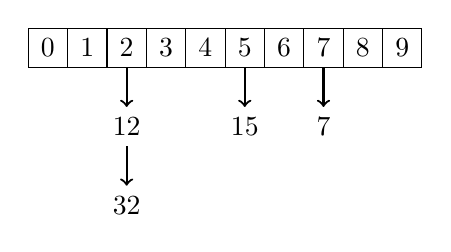
\begin{tikzpicture}[scale=0.5]
\draw (0,0) grid (10,1);
\foreach \x in {0,1,...,9} \node at (0.5+\x,0.5) {\x};
\draw[->,thick] (2.5,0) -- (2.5,-1);
\draw[->,thick] (5.5,0) -- (5.5,-1);
\draw[->,thick] (7.5,0) -- (7.5,-1);
\draw[->,thick] (2.5,-2) -- (2.5,-3);
\node at (2.5,-1.5) {$12$};
\node at (5.5,-1.5) {$15$};
\node at (7.5,-1.5) {$7$};
\node at (2.5,-3.5) {$32$};
\end{tikzpicture}
\caption{Hajautustaulu, joka vastaa joukkoa $\{7,12,15,32\}$.
Hajautusfunktiona on $f(x)=x \bmod 10$.}
\label{fig:hajtau}
\end{figure}

Kuvassa \ref{fig:hajtau} on esimerkkinä hajautustaulu,
jonka kokona on $N=10$.
Olemme tallentaneet hajautustauluun joukon $\{7,12,15,32\}$
käyttäen yksinkertaista hajautusfunktiota $f(x)=x \bmod 10$.
Tämä tarkoittaa, että alkion $x$ hajautusarvo on sen jakojäännös $10$:llä
eli luvun viimeinen numero.
Esimerkiksi alkiot $12$ ja $32$ ovat kohdassa $2$,
koska niissä viimeinen numero on $2$,
ja alkiot $15$ ja $7$ ovat vastaavasti kohdissa $5$ ja $7$.
Kaikki muut hajautustaulun listat ovat tällä hetkellä tyhjiä.

Kun haluamme tarkistaa, onko joukossa alkiota $x$,
laskemme ensin sen hajautusarvon $f(x)$.
Tämän jälkeen käymme läpi kaikki kohdan $f(x)$
listassa olevat alkiot ja tarkistamme,
onko jokin niistä alkio $x$.
Vastaavasti kun haluamme lisätä alkion $x$ joukkoon
tai poistaa alkion $x$ joukosta,
teemme muutoksen kohdassa $f(x)$ olevaan listaan.
Nämä operaatiot vievät aikaa $O(m)$,
kun $m$ on hajautustaulussa olevan listan pituus.
Tavoitteemme on, että kaikissa listoissa $m$ on pieni,
jolloin operaatiot toimivat tehokkaasti.

\subsection{Hajautusfunktio}

Hajautusfunktio $f(x)$ määrittää, mihin kohtaan hajautustaulua
alkio $x$ sijoitetaan.
Sen täytyy antaa jokaiselle mahdolliselle alkiolle
hajautusarvo eli kokonaisluku väliltä $0,1,\dots,N-1$,
missä $N$ on hajautustaulun koko.
Lisäksi jotta hajautustaulu olisi käyttökelpoinen,
hajautusfunktion tulisi jakaa alkiot
\emph{tasaisesti} eri puolille hajautustaulua.
Tällöin hajautustaulun listat ovat lyhyitä ja
operaatiot toimivat tehokkaasti.

\begin{figure}
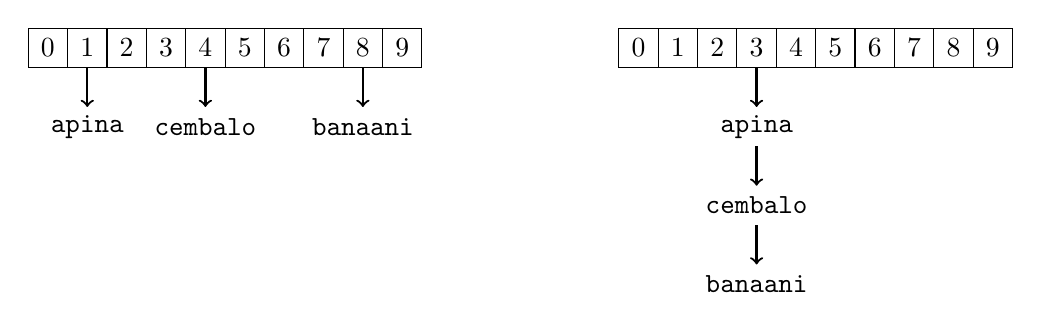
\begin{tikzpicture}[scale=0.5]
\begin{scope}
\draw (0,0) grid (10,1);
\foreach \x in {0,1,...,9} \node at (0.5+\x,0.5) {\x};
\draw[->,thick] (1.5,0) -- (1.5,-1);
\draw[->,thick] (4.5,0) -- (4.5,-1);
\draw[->,thick] (8.5,0) -- (8.5,-1);
\node at (1.5,-1.5) {\texttt{apina}};
\node at (8.5,-1.5) {\texttt{banaani}};
\node at (4.5,-1.5) {\texttt{cembalo}};
\end{scope}
\begin{scope}[xshift=15cm]
\draw (0,0) grid (10,1);
\foreach \x in {0,1,...,9} \node at (0.5+\x,0.5) {\x};
\draw[->,thick] (3.5,0) -- (3.5,-1);
\draw[->,thick] (3.5,-4) -- (3.5,-5);
\draw[->,thick] (3.5,-2) -- (3.5,-3);
\node at (3.5,-1.5) {\texttt{apina}};
\node at (3.5,-5.5) {\texttt{banaani}};
\node at (3.5,-3.5) {\texttt{cembalo}};
\end{scope}
\end{tikzpicture}
\caption{Kaksi hajautustaulua joukolle $\{\texttt{apina},\texttt{banaani},\texttt{cembalo}\}$.
Vasemmassa taulussa hajautus on onnistunut täydellisesti,
oikeassa taulussa kaikki alkiot ovat samassa listassa.}
\label{fig:hajjak}
\end{figure}

Kuva \ref{fig:hajjak} näyttää kaksi hajautustaulua, jotka vastaavat
samaa joukkoa kahdella eri hajautusfunktiolla.
Vasemmassa taulussa hajautus on onnistunut täydellisesti
ja jokainen alkio on omassa listassaan.
Oikeassa taulussa taas kaikki alkiot ovat joutuneet samaan
listaan eikä hajautuksesta ole mitään hyötyä.
Tavoitteemme on, että saisimme aikaan hajautusfunktion,
jonka toiminta on lähempänä vasenta taulua.

Tarkastelemme seuraavaksi esimerkkinä hajautusfunktioita,
joiden avulla voi laskea hajautusarvon merkkijonolle.
Meidän riittää määritellä hajautusfunktio,
joka muuttaa merkkijonon epänegatiiviseksi kokonaisluvuksi,
koska tämän jälkeen saamme helposti kokonaisluvun
väliltä $0 \dots N-1$ ottamalla alkuperäisestä luvusta jakojäännöksen $N$:llä.

Oletamme, että merkkijonossa on $k$ merkkiä,
joiden merkkikoodit\footnote{Käytämme tässä merkkien ASCII-koodeja.
Esimerkiksi Javassa char-merkin \texttt{c} koodin saa
selville kirjoittamalla \texttt{(int)c}, eli esimerkiksi
\texttt{(int)'a'} on 97.} ovat $c_0,c_1,\dots,c_{k-1}$.
Esimerkiksi jos merkkijono on \texttt{apina},
$k=5$ ja koodit ovat $c_0=97$, $c_1=112$, $c_2=105$,
$c_3=110$ ja $c_4=97$.
Seuraavassa on kolme mahdollista tapaa määritellä hajautusfunktio:

\begin{enumerate}
\item Hajautusarvo on merkkijonon pituus $k$.
Esimerkiksi merkkijonon \texttt{apina} hajautusarvo on 5.
\item Hajautusarvo on merkkikoodien summa
\[ c_0 + c_1 + \dots + c_{k-1}.\]
Esimerkiksi merkkijonon \texttt{apina} hajautusarvo on
\[97+112+105+110+97=521.\]
\item Hajautusarvo on summa
\[ A^{k-1} c_0 + A^{k-2} c_1 + \dots + A^0 c_{k-1},\]
missä $A$ on vakio (\emph{polynominen hajautus}).
Esimerkiksi jos $A=7$, merkkijonon \texttt{apina} hajautusarvo on
\[7^4 \cdot 97+7^3 \cdot 112+7^2 \cdot 105+7^1 \cdot 110+7^0 \cdot 97=61235.\]
\end{enumerate}

Funktiot 1 ja 2 eivät ole käytännössä hyviä hajautusfunktioita,
koska ne antavat saman hajautusarvon monille merkkijonoille.
Funktio 1 antaa kahdelle merkkijonolle saman hajautusarvon,
jos ne ovat yhtä pitkiä,
ja funktio 2 antaa kahdelle merkkijonolle saman hajautusarvon,
jos ne sisältävät samat merkit eri järjestyksessä.

Funktio 3, jota kutsutaan nimellä polynominen hajautus,
on käytännössä hyvä hajautustapa, joka on käytössä esimerkiksi
Javan standardikirjastossa.
Vakio $A$ valitaan tyypillisesti niin, että se on pieni alkuluku.
Koska hajautusarvo lasketaan painotettuna summana,
kaksi eri merkkijonoa eivät yleensä saa samaa hajautusarvoa.
Toisaalta pystymme laskemaan hajautusarvon tehokkaasti
mille tahansa merkkijonolle.

\subsection{Hajautuksen tehokkuus}

Hajautustaulun operaatiot vievät aikaa $O(m)$,
jossa $m$ on pisimmän listan pituus.
Mutta kuinka suuri $m$ on? Tämä riippuu siitä,
mikä on alkioiden määrä $n$, hajautustaulun koko $N$
sekä hajautusfunktio $f$.

Jos kaikki sujuu hyvin ja hajautusfunktio jakaa alkioita
tasaisesti hajautustaulun eri puolille,
jokaisessa listassa on noin $n/N$ alkiota.
Niinpä jos valitsemme hajautustaulun koon niin,
että $N$ on samaa luokkaa kuin $n$,
operaatiot toimivat tehokkaasti ajassa $O(1)$.
Kuitenkin on mahdollista että hajautus epäonnistuu
ja alkiot jakautuvat hajautustauluun epätasaisesti.
Pahimmassa tapauksessa kaikki alkiot saavat saman
hajautusarvon ja ne kaikki tallennetaan samaan listaan,
jolloin operaatiot vievät aikaa $O(n)$.

Voimme helposti vaikuttaa hajautustaulun kokoon $N$,
mutta hajautusfunktion suunnittelu on epämääräisempi ala.
Miten voimme tietää, että valitsemamme hajautusfunktio
toimii hyvin?
Tämä on hyvä kysymys ja luvussa 6.4
paneudumme asiaan tarkemmin tutkimalla polynomisen
hajautuksen toimivuutta todellisella aineistolla.

Toisaalta vaikka meillä olisi erittäin hyvä hajautusfunktio,
\emph{ilkeä vastustaja} voi kuitenkin antaa
meille joukon alkioita, jotka kaikki saavat saman hajautusarvon.
Ilkeä vastustaja tarkoittaa kuvitteellista tai todellista vihollista,
joka paljastaa heikkouden hajautusfunktiossamme.
Tämä riski on aina hajautuksessa, koska mahdollisten
hajautusarvojen määrä on pienempi kuin mahdollisten alkioiden määrä
eikä ole mahdollista toteuttaa hajautusfunktiota niin,
että se jakaisi alkiot \emph{varmasti} tasaisesti hajautustauluun.

Kaikeksi onneksi hajautus toimii yleensä aina \emph{käytännössä}
hyvin ja voimme ajatella, että hajautustaulun operaatiot ovat
$O(1)$-aikaisia.
Vaikka on mahdollista, että hajautus epäonnistuu,
tämän riski on niin pieni, että meidän ei tarvitse murehtia
siitä käytännössä.

\section{Hajautus Javassa}

Javassa on kaksi hajautustaulua käyttävää tietorakennetta:
\texttt{HashSet} pitää yllä alkioiden joukkoa
hajautustaulun avulla, ja \texttt{HashMap} säilyttää
joukkoa avain-arvo-pareja, mitä voi ajatella taulukon yleistyksenä.
Seuraavaksi tutustumme tarkemmin näihin rakenteisiin.

\subsection{\texttt{HashSet}-rakenne}

Javan \texttt{HashSet}-rakenne pitää yllä joukkoa alkioista.
Joukkoon voi lisätä alkion metodilla \texttt{add},
ja siitä voi poistaa alkion metodilla \texttt{remove}.
Esimerkiksi seuraava koodi luo joukon, jossa voi olla
kokonaislukuja, ja lisää siihen luvut 3, 5 ja 8.
Tämän jälkeen koodi poistaa luvun 5 joukosta.

\begin{code}
HashSet<Integer> joukko = new HashSet<>();
joukko.add(3);
joukko.add(5);
joukko.add(8);
System.out.println(joukko); // [3, 5, 8]
joukko.remove(5);
System.out.println(joukko); // [3, 8]
\end{code}

Metodin \texttt{contains} avulla voimme selvittää,
esiintyykö tietty alkio joukossa:

\begin{code}
if (joukko.contains(5)) {
    System.out.println("Luku 5 on joukossa");
}
\end{code}

Huomaa, että jokainen alkio voi esiintyä vain kerran joukossa.
Esimerkiksi vaikka seuraava koodi lisää luvun 5 kolmesti
joukkoon, se menee sinne vain ensimmäisellä kerralla ja
muut lisäykset jätetään huomiotta.

\begin{code}
HashSet<Integer> joukko = new HashSet<>();
joukko.add(5);
joukko.add(5);
joukko.add(5);
System.out.println(joukko); // [5]
\end{code}

\subsection{\texttt{HashMap}-rakenne}

\texttt{HashMap}-rakenne pitää yllä joukkoa avain-arvo-pareja.
Rakennetta voi ajatella taulukon yleistyksenä:
$n$ alkion taulukossa avaimet ovat aina kokonaisluvut
$0,1,\ldots,n-1$, mutta \texttt{HashMap} sallii
avaimina minkä tahansa tyyppisiä alkioita eikä niiden
tarvitse olla peräkkäisiä kokonaislukuja.

\texttt{HashMap}-rakenteen määrittelyssä tulee antaa
avaimen ja arvon tyyppi.
Esimerkiksi seuraava koodi luo sanakirjan, jossa sekä
avaimet että arvot ovat merkkijonoja.
Syötämme sanakirjaan merkkijonopareja, jotka kertovat
sanan käännöksen suomesta englanniksi.
Metodi \texttt{put} lisää uuden avain-arvo-parin,
ja metodi \texttt{get} hakee arvon avaimen perusteella.

\begin{code}
HashMap<String,String> sanakirja = new HashMap<>();

sanakirja.put("apina","monkey");
sanakirja.put("banaani","banana");
sanakirja.put("cembalo","harpsichord");

System.out.println(sanakirja.get("banaani")); // banana
\end{code}

Hyödyllinen on myös metodi \texttt{containsKey},
jonka avulla voi tarkastaa, onko tietylle avaimelle
tallennettu arvoa:

\begin{code}
if (sanakirja.containsKey(sana)) {
    System.out.println("Käännös: " + sanakirja.get(sana));
} else {
    System.out.println("Sana puuttuu sanakirjasta!");
}
\end{code}

Koska \texttt{HashMap} on toteutettu hajautustaulun avulla,
sen operaatiot toimivat tehokkaasti keskimäärin $O(1)$-ajassa.

\subsection{Omat luokat}

Javan olioissa on metodi \texttt{hashCode},
jonka avulla olio kertoo pyydettäessä hajautusarvonsa.
Voimme esimerkiksi selvittää merkkijonon \texttt{apina}
hajautusarvon seuraavasti:

\begin{code}
System.out.println("apina".hashCode());
\end{code}

Tämä koodi tulostaa luvun 93022541,
joka on siis merkkijonon \texttt{apina} hajautusarvo Javassa.
On tunnettua, että Java käyttää merkkijonon hajautusarvon laskemiseen
polynomista hajautusta vakiolla $A=31$,
joten voimme laskea Javan hajautusarvon myös itse kaavalla
\[31^4 \cdot 97+31^3 \cdot 112+31^2 \cdot 105+31^1 \cdot 110+31^0 \cdot 97=93022541.\]

Jos haluamme käyttää omia oliota hajautustauluissa,
meidän täytyy toteuttaa luokkaan kaksi metodia:
\texttt{hashCode}, joka antaa olion hajautusarvon,
sekä \texttt{equals},
joka ilmaisee, ovatko kaksi oliota samat.
Jälkimmäinen metodi on tarpeen,
jotta Java pystyy varmistamaan, ovatko saman hajautusarvon
antavat oliot todella samat.


Esimerkiksi jos meillä on luokka \texttt{Piste},
jossa on kenttinä kokonaisluvut \texttt{x} ja \texttt{y},
voisimme toteuttaa metodit seuraavasti:

\begin{code}
class Piste {
    public int x, y;

    public int hashCode() {
        return 97*x+y;
    }
    
    public boolean equals(Object o) {
        Piste p = (Piste)o;
        return x == p.x && y == p.y;
    }

    // ...
}
\end{code}

Tässä toteutuksessa siis pisteen $(x,y)$ hajautusarvo lasketaan
kaavalla $97x+y$, missä 97 on valitsemamme vakio, jolla ei ole
syvällistä merkitystä.
Nyt kun hajautusfunktio on kunnossa,
voimme luoda vaikkapa \texttt{HashSet}-rakenteen, jossa on pisteitä:

\begin{code}
HashSet<Piste> joukko = new HashSet<Piste>();
joukko.add(new Piste(3,2));
joukko.add(new Piste(1,4));
joukko.add(new Piste(1,3));
\end{code}

\section{Esimerkki: Anagrammit}

Annettuna on lista sanoja ja haluamme jakaa sanat ryhmiin niin,
että kukin ryhmä sisältää sanat, jotka ovat keskenään anagrammeja.
Kaksi sanaa ovat anagrammit, jos ne on mahdollista muuttaa toisikseen
muuttamalla niiden kirjainten järjestystä.

Esimerkiksi jos sanat ovat ''abc'', ''iines'', ''bac'', ''cba'' ja ''sieni'',
niistä muodostuu kaksi ryhmää.
Ensimmäisessä ryhmässä on sanat ''abc'', ''bac'' ja ''cba'',
ja toisessa ryhmässä on sanat ''iines'' ja ''sieni''.

Voimme ratkaista tehtävän tehokkaasti seuraavan havainnon avulla:
jos kaksi sanaa ovat anagrammit ja järjestämme niiden kirjaimet,
ne muuttuvat samoiksi.
Esimerkiksi sanoissa ''iines'' ja ''sieni'' kirjaimet
järjestettyinä ovat ''eiins''.
Tämän havainnon ansiosta voimme käyttää kunkin anagrammiryhmän
tunnuksena sen sanojen järjestettyä muotoa.

Luomme ryhmiä varten rakenteen

\begin{code}
HashMap<String,ArrayList<String>> ryhmat = new HashMap<>();
\end{code}

jossa avaimena on anagrammiryhmän tunnus ja arvona on lista,
joka sisältää kaikki listaan kuuluvat sanat.
Algoritmin runko näyttää seuraavalta, kun oletamme,
että sanat on tallennettu listaan \texttt{sanat}:

\begin{code}
for (String sana : sanat) {
    String avain = tunnus(sana);
    if (!ryhmat.containsKey(avain)) {
        ryhmat.put(avain,new ArrayList<>());
    }
    ryhmat.get(avain).add(sana);
}
System.out.println(ryhmat);
\end{code}

Tarvitsemme vielä metodin \texttt{tunnus}, joka järjestää
sanan kirjaimet aakkosjärjestykseen.
Jotta voimme järjestää sanan, muutamme sen merkkitaulukoksi,
järjestämme taulukon, ja palautamme sitten uuden merkkijonon,
joka on muodostettu taulukosta.

\begin{code}
String tunnus(String sana) {
    char[] taulu = sana.toCharArray();
    Arrays.sort(taulu);
    return new String(taulu);
}
\end{code}

Esimerkin tapauksessa ohjelmamme tulostus on seuraava:

\begin{code}
{abc=[abc, bac, cba], eiins=[iines, sieni]}
\end{code}

\section{Hajautuksen parametrit}

TODO